\chapter{Entity Calculus}\label{ch:entitycalc} 
In this module system, I will use an entity calculus, a refined
version of the static representation of functor actions and static
module content found in the SML/NJ compiler. The entity calculus
provides a natural representation of the static content of modules,
which I call \emph{static entities}. The term entity refers to an
extended\footnote{Entity calculus tycons differ from syntactic types
  only in that the tycons may have been relativized, a process
  described in a later section, and prefixed polymorphic (universal) quantifiers.}
form of type constructors ($\mathbb{C}^\lambda$) and a static
description of objects that may include type constructors such as
structures and functors. In the module system, syntactic signatures
alone are insufficient for expressing functor actions. The entity
calculus is a small language for expression exactly that, the functor
actions for a functor. 
   
\input{../design/figs/fig-rlzn}
   
Fig.~\ref{fig:entities} describes the entity calculus, comprising of
entity expressions $\varphi$, entity declarations $\eta$, and static
entities $\upsilon$. The static entities are the entity calculus
analogue to values in the lambda calculus. The representation relies
on a denumerable set of variables, EntityVars, which represents unique names that can be thought of as the new variable names resulting from alpha-conversion.
  
Entity environments $\Upsilon$ are sequences of bindings of an entity
variable $\rho$ to a static entity $\upsilon$. The sequence is
important because the semantics needs a deterministic way to search
through the environment for atomic tycons. The role of entity environments is two-fold. They give the
current instantiation of a relativized tycon, thus enabling
translation of a relativized tycon to a specific semantic
tycon. Furthermore, they permit the translation of a semantic tycon
back to an entity path, a canonical relativized tycon. 
     
There are four forms of static entities, corresponding to structure, functor, atomic tycons, and definitional
(derived) tycons. Structure and functor entities are enclosed in
$\langle\rangle$ brackets. A structure entity
$\langle\Upsilon^{lcl},\Upsilon^{clo} \rangle$ has a
local entity environment $\Upsilon^{lcl}$ and a closure environment
$\Upsilon^{clo}$ to close an associated semantic signature with respect to any entity variable not defined in $\Upsilon^{lcl}$, \ie, the nonlocal entity variables. 

\begin{lstlisting}
signature S = 
sig
  type t
  structure S' = sig val x : t end
end

structure M =
struct
  type t = int
  structure S ' = struct val x = 1 end
end
\end{lstlisting}

Consider the above example. The semantic signature S' has a free occurrence of the entity variable for t $\rho_t$. The entity variable $\rho_t$ is not in the domain of the entity environment for S'. In fact, the entity environment for S' is empty because S' does not contain any static entities. Still, the structure entity for S' must be self-contained. Therefore it must close the signature for S' with a closure entity environment which is a copy of the entity environment for its enclosing structure.  A structure entity encodes only the volatile type information in structure, \ie, the part that is re-instantiated with signature matching and functor application. 

There are two forms of functor entity. The standard form
$\langle\lambda\rho.\varphi;\Upsilon\rangle$ encodes the functor
action as an \emph{entity function} $\lambda\rho.\varphi$ together with a closure
entity environment $\Upsilon$. Applying an entity function results in a structure entity. The alternate form
$\langle\lambda\rho.\Sigma;\Upsilon\rangle$ 
represent functors in formal functor parameters where the
only information known is the semantic signature $\Sigma$ of the functor result, described in chapter~\ref{ch:homods} in fig.~\ref{fig:semanticobjs}. Semantic signatures
are syntactic signatures where each of the static
components (tycons, structures, and functors) are decorated with
entity variables. They are formally defined in chapter~\ref{ch:homods}. A semantic signature may mention entities by their entity variables (called \emph{relativized} tycons), hence it must closed by an entity environment $\Upsilon$. Relativization is formally defined in sec.~\ref{sec:relativization}. Atomic tycons
$\tau^n$ and definitional tycons $\mathfrak{C}^\lambda$
(defined in sec.~\ref{sec:relativized-type-sys}) are
the tycon entities. Entity environments may contain definitional tycons because of signature matching, a subject thoroughly discussed in sec.~\ref{sec:sigmatch}. 

Static entities are the values computed by the entity calculus. Tycon entity expressions evaluate to tycon entities. Previously declared tycons and formal tycons from functor parameters are represented by their entity path, $\vec{\rho}$. They can also be a $\newx(n)$ or a relativized tycon $\mathbb{C}^\lambda$ (defined in sec.~\ref{sec:relativization}) that refers to a tycon whose instantiation is in an entity environment. The $\newx(n)$ form produces a new atomic tycon $\tau^n$ when evaluated where $n$ specifies the arity of the desired tycon. The $\newx(n)$ expression is the key to representing type generativity in the entity calculus. Datatypes and other generative tycons are represented by the form $\newx(n)$ which when evaluated will generate a fresh type constructor unequal to all those generated before it. 

Structure entity expressions and functor entity expressions evaluate to
structure entities and functor entities respectively. The entity path
form in both structure and functor entity expressions is a reference
to an entity bound in a previous entity declaration. Structure entity
expressions also consist of entity declarations enclosed by
$\llparenthesis\cdot\rrparenthesis$ corresponding to the
\lstinline{struct ... end} base structure form, functor application expressions, and 
let expressions. The let expression is used to express coercions induced by
signature matching (see sec.~\ref{sec:sigmatch}). In addition to an
entity path, functor entity expressions may be entity lambda abstractions or 
formal functors of the form $\lambda\rho.\Sigma$. 
 
Entity declarations bind an entity variable to tycon entity expressions, structure entity
expressions, and functor entity expressions. The entity calculus has a static compile-time semantics. The elaborator evaluates entity expressions to static entities as necessary during elaboration. The judgments for the entity expression evaluation are outlined below:
 
\begin{tabular}{ll}
	$\Upsilon\vdash\varphi \Downarrow_{str} R$ & structure entity expression evaluation \\
	$\Upsilon\vdash\eta \Downarrow_{decl} \Upsilon'$ & entity declaration evaluation \\
	$\Upsilon\vdash\theta \Downarrow_{fct} \psi$ & functor entity expression evaluation
\end{tabular}

$\Upsilon$ is an entity environment. $\varphi$ is the resulting entity expression.  $\psi$ is a resulting functor entity. $R$ is the entity environment obtained by evaluating the structure entity expression. $\Upsilon'$ is the entity environment obtained by evaluating the entity declarations $\eta$. Each binding in $\Upsilon'$ corresponds to an entity declaration in $\eta$, thus $\Upsilon\not\subseteq\Upsilon'$. 

\section{Entity declarations}
The evaluation rules for entity declarations must accumulate the entity environment across declarations in order to support occurrences of entities in value specs within inline open signatures. 

\begin{singlespace}
\begin{lstlisting}
datatype d = A

structure M : sig type t val x : d * t end =
struct
  datatype t = B
  val x = (A, B)
end
\end{lstlisting}
\end{singlespace}

Observe that the type name d is a nonlocal name that must be defined in a prior entity declaration. The clause entity environment for M must contain a binding for d.  

\section{Notation}\label{sec:entitycalc-notation}
I indicate extension of entity environments by juxtaposition, $\Upsilon[\rho\mapsto\upsilon]$. This notation should never cause shadowing of entity variable bindings because the convention is that $\rho\notin dom(\Upsilon)$. 
Entity environment concatenation of two entity environments $\Upsilon$ and $\Upsilon'$ is represented by juxtaposition, $\Upsilon\Upsilon'$. The notation for entity environment lookup is overloaded. $\Upsilon(\rho)$ looks up the static entity corresponding to $\rho$. The notation $\Upsilon(\rho_0\vec{\rho})$ looks up $\rho_0$ in $\Upsilon$ for a structure entity $R=\langle \Upsilon^{lcl},\Upsilon^{clo} \rangle$ and then recursively computes $\Upsilon'(\vec{\rho})$ such that $\Upsilon' = \Upsilon^{clo}\Upsilon^{lcl}$. Let $EV(\cdot)$ denote the set of all entity variables in $\cdot$. The notation $dom(\Upsilon)$ denotes the set of entity variables in the domain of all mappings in $\Upsilon$, including the nested ones. 

Let $R$ be a structure entity $\langle\Upsilon^{lcl},\Upsilon^{clo}\rangle$ and $\vec{\rho}$ be an entity path defined in either $\Upsilon^{lcl}$ or $\Upsilon^{clo}$. Then $R(\vec{\rho})$ is defined such that $R(\vec{\rho}) = \Upsilon^{clo}\Upsilon^{lcl}(\vec{\rho})$. 

$\Upsilon_1 \subseteq \Upsilon_2$ indicates all the bindings in
$\Upsilon_1$ are in $\Upsilon_2$. The notation $R \subseteq \Upsilon$
means $\Upsilon^{clo}\Upsilon^{lcl}\subseteq \Upsilon$ where $R=\langle
\Upsilon^{lcl}, \Upsilon^{clo}\rangle$. Similarly, $\Upsilon\subseteq R$
indicates $\Upsilon \subseteq \Upsilon^{clo}\Upsilon^{lcl}$. The convention that that if $R$ is used in a place where an entity environment is expected, then $R$ denotes $\Upsilon^{clo}\Upsilon^{lcl}$ such that $R = \langle \Upsilon^{lcl}, \Upsilon^{clo} \rangle$. 

\section{Entity Evaluation Semantics}
\input{../design/figs/fig-evalent}

Entity declarations evaluate to entity environments. The module system evaluates entity expressions when elaborating functor application (rule \ref{eq:strapp}). Each entity expression represents the latent static computation in a structure or functor expression. Once evaluated, the resultant structure entity provides a precise and complete (closed) description of the entities inside a structure. Evaluation requires an entity environment as context to interpret entity paths in the entity expressions and declarations. 

Fig.~\ref{fig:entsems} lists the rules for evaluating entity expressions. The key rules are the ones for application (\ref{eq:expapp}). There are two, one for regular functor application and the other for formal functor application. The functor entity expression is evaluated to an entity function. The argument structure entity expression is evaluated to an entity environment. The body of the entity function is then evaluated in an entity environment extended with the closure environment and the formal parameter entity variable mapped to the argument structure entity environment. Rule~\ref{eq:expappformal} evaluates the functor entity expression to a functor entity corresponding to the formal functor case and also the structure entity expression to the structure entity. The semantic signature $\Sigma$ (\ie~the formal functor body signature) must be instantiated (a process that is covered in sec.~\ref{sec:siginst}). The rule then forms a structure entity using this instantiation and the extended entity environment as a closure. The instantiation part of the closure will correspond to the actual functor closure when the actual functor is known. 

%!TEX root = ../principles.tex
\begin{figure}
\centering

\fixedCodeFrame{
\small
~\\[0.5mm]
\fbox{$\Upsilon\vdash \eta \Downarrow_{decl} \Upsilon'$}
\begin{equation}
	\infer{\Upsilon\vdash\bullet\Downarrow_{decl} \emptyset_{ee}}
        {\strut}
\label{eq:entdecempty}
\end{equation}

\begin{equation}
	 \infer{\Upsilon\vdash\rho=_{str}\varphi,\eta\Downarrow_{decl}[\rho\mapsto R]\Upsilon'}
	{\Upsilon\vdash\varphi\Downarrow_{str}R\qquad 
          \Upsilon[\rho\mapsto R]\vdash\eta\Downarrow_{decl}
          \Upsilon'} 
\label{eq:entdecstr}
\end{equation}
	
\begin{equation}
	\infer{\Upsilon\vdash\rho=_{fct}\theta,\eta\Downarrow_{decl}[\rho\mapsto\psi]\Upsilon'}
	  {\Upsilon\vdash\theta\Downarrow_{fct}\psi\qquad 
            \Upsilon[\rho\mapsto\psi]\vdash\eta\Downarrow_{decl}
            \Upsilon'}
\label{eq:entdecfct}
\end{equation}

\begin{equation}
	\infer{\Upsilon\vdash\rho=_{tyc}\newx(n),\eta\Downarrow_{decl}
          [\rho\mapsto\tau^n]\Upsilon'}
	    {\begin{array}{c}
                \Upsilon[\rho\mapsto\tau^n]\vdash\eta\Downarrow_{decl}\Upsilon'\qquad
            (\tau\textrm{ is fresh in }\Upsilon)
          \end{array}} 
\label{eq:entdecnew}
\end{equation}

\begin{equation}
         \infer{\Upsilon\vdash[\rho=_{def}\mathbb{C}^\lambda],\eta\Downarrow_{decl}
           [\rho\mapsto\mathbb{C}^\lambda]\Upsilon'}
         {\Upsilon[\rho\mapsto\mathbb{C}^\lambda]\vdash\eta\Downarrow_{decl}
           \Upsilon'}
         \label{eq:entdectypedef}
\end{equation}

\begin{equation}
         \infer{\Upsilon\vdash[\rho=_{def}\vec{\rho}],\eta\Downarrow_{decl}
           [\rho\mapsto\Upsilon(\vec{\rho})]\Upsilon'}
         {\Upsilon[\rho\mapsto\Upsilon(\vec{\rho})]\vdash \eta
           \Downarrow_{decl} \Upsilon'}
         \label{eq:entdecalias}
\end{equation}
}
\caption{Entity declaration semantics}
\label{fig:entdecsems}
\end{figure}
Entity declarations must be evaluated in
sequence. Fig.~\ref{fig:entdecsems} formally defines how to evaluate
entity declarations. Each tycon, structure, and functor entity declaration evaluates the respective tycon, structure entity expression, and functor entity expression to the corresponding entity. The subsequent entity declarations are evaluated in the context of an entity environment extended with a mapping for that entity. The entity environment context only has bindings for the entity variables bound in the entity declarations because only entity expression evaluation will provide the correct closure.

Rule~\ref{eq:entdecempty} ensures that the resultant entity
environment is cumulative. Rules~\ref{eq:entdecstr}
and~\ref{eq:entdecfct} evaluate structure and functor entity
declarations in the expected way.  Rule~\ref{eq:entdecnew} is the key
rule that generates fresh atomic tycons with the appropriate arity
$n$. When the $\rho=_{tyc}\newx(n)$ entity declaration is embedded in
the body of a functor entity, it produces a fresh atomic tycon for
$\rho$ each time the functor entity is applied,\ie~also when this
entity declaration is evaluated. This models exactly the behavior of
generative datatype declarations under true higher-order
semantics. Rule~\ref{eq:entdectypedef} yields a corresponding type
definition entity environment binding. Rule~\ref{eq:entdecalias} looks
up an entity path (constructed during signature matching coercion
rule~\ref{eq:coerceopen}) for the corresponding entity mapping. 
  
%!TEX root = ../principles.tex
\begin{figure}
\centering
\fixedCodeFrame{
\small
~\\[2mm]
\fbox{$\Upsilon\vdash\theta\Downarrow_{fct}\psi$}
\begin{equation}
\infer{\Upsilon\vdash\vec{\rho}\Downarrow_{fct}\Upsilon(\vec{\rho})}
{\strut} 
\label{eq:fctentpath}
\end{equation}

\begin{equation}
\infer{\Upsilon\vdash\lambda\rho.\varphi
\Downarrow_{fct}\langle
  \lambda\rho.\varphi;\Upsilon\rangle}
{\strut}	
\label{eq:fctentlam}
\end{equation}

\begin{equation}
\infer{\Upsilon\vdash\lambda\rho.\Sigma \Downarrow_{fct} \langle
  \lambda\rho.\Sigma; \Upsilon
  \rangle}
{\strut}
\label{eq:fctentformal}
\end{equation}

}
\caption{Functor entity evaluation}
\label{fig:fctenteval}
\end{figure}
 
Fig.~\ref{fig:fctenteval} gives the rules for evaluating a functor entity expression. Rule~\ref{eq:fctentpath} looks up entity paths in the usual way. The entity function is formed by combining an entity $\lambda$-abstraction with the current entity environment to form a closure (rule~\ref{eq:fctentlam}). Rule~\ref{eq:fctentformal} similarly forms a closure for formal functors.  

\begin{lemma}[Entity evaluation terminates]
The following evaluation relations terminate (have a finite derivation tree):
\begin{enumerate}
\item $\Upsilon\vdash\varphi\Downarrow_{str}R$
\item $\Upsilon\vdash\eta\Downarrow_{decl}\Upsilon'$
\item $\Upsilon\vdash\theta\Downarrow_{fct} \psi$
\end{enumerate}
\end{lemma}

\begin{lemma}
\begin{enumerate}
\item If $\Upsilon \vdash \varphi \Downarrow_{str} R$, then
$\Upsilon\subseteq R$.
\item If $\Upsilon\vdash \theta \Downarrow_{fct}
\langle\theta;\Upsilon'\rangle$, then $\Upsilon\subseteq\Upsilon'$. 
\end{enumerate}
\end{lemma}

\section{Relativization}\label{sec:relativization}
Tycon names have a scoping policy much like other program identifiers. Tycon names can be shadowed by later tycon declarations. A tycon name may refer to a local tycon that is declared in the same semantic signature or structure entity, or to a nonlocal one that is declared as a functor parameter or in another structure. Although signature declarations occur only at the top level, anonymous signature expressions may be embedded as functor parameter signatures and signature ascriptions. When signatures occur inline, its type specifications may refer to both local and nonlocal tycons.

Some tycon names may refer to volatile tycons which may be instantiated multiple times possibly to new generative tycon. Each time a functor is applied or a structure is ascribed a signature, the tycon name must be interpreted according to a potentially different entity environment. When elaboration reaches these tycons we need a way to map them back to the corresponding entity path such that we reference the correct ``up-to-date'' volatile tycon. The necessity of this is illustrated in fig.~\ref{fig:lifecycle}. Semantic tycons which live in static environments and entity environments have to be relativized when put into semantic signatures and entity expressions. When the tycon is needed for typechecking, the tycon must be instantiated with respect to an entity environment. This is the primary purpose of relativization, to give an entity path that can be interpreted according to different entity environments. Secondarily, relativization replaces fragile symbolic names with robust entity paths to the entity environment mapping the entity paths. 

\begin{figure}
\begin{center}
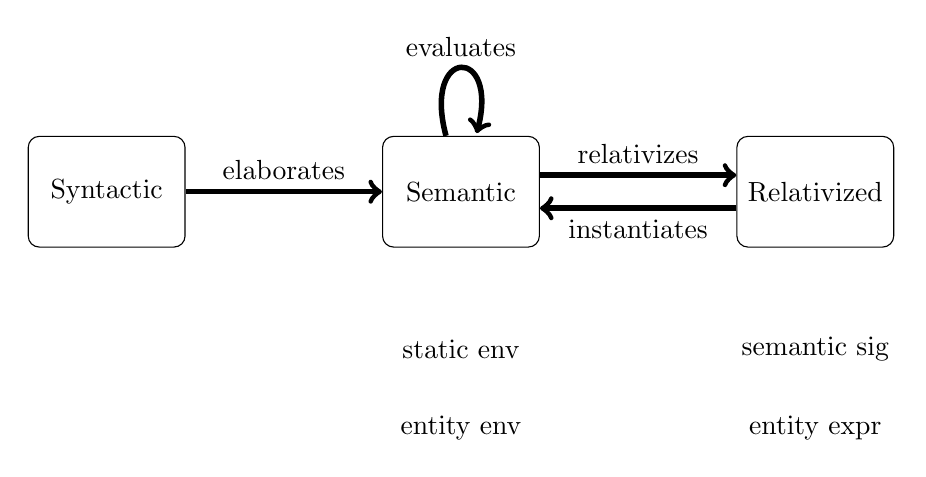
\begin{tikzpicture}[node distance= 4.5cm,auto]
\tikzstyle{block} = [rectangle, draw,  
    text width=5em, text centered, rounded corners, minimum height=4em]
\tikzstyle{arr} = [line width=2pt,->]
	\node[block] (sy) {Syntactic};
	\node[block, right of=sy] (se) {Semantic};
	\node[block, right of=se] (re) {Relativized};

	\node[node distance=2cm,below of=se] (statenv) {static env};
	\node[node distance=1cm,,below of=statenv] {entity env};
	\node[node distance=2cm,below of=re] (semsig) {semantic sig};
	\node[node distance=1cm,below of=semsig]  {entity expr};
		
	\path[arr] (sy) edge node {elaborates} (se);
	\path[arr] ([yshift=-5mm]se.north east) edge node {relativizes} ([yshift=-5mm]re.north west);
	\path[arr] (se) edge [loop above] node {evaluates} (se);
	\path[arr] ([yshift=5mm]re.south west) edge node {instantiates} ([yshift=5mm]se.south east);
	

\end{tikzpicture}
\end{center}
\caption{Life-cycle of a tycon}
\label{fig:lifecycle}
\end{figure}

\subsection{Relativized Type System}\label{sec:relativized-type-sys}
\begin{figure}
	\hrule
\[\begin{array}{rcll}
       \mathbb{C}^s & ::= &
         \alpha~|~\vec{\rho}(\vv{\mathbb{C}^s}) & \textrm{relativized monotypes}\\
       \mathbb{C}^\lambda & ::= & \lambda\vec{\alpha}.\mathbb{C}^s &
       \textrm{relativized tycons}\\

        \mathbb{T} & ::= &
        \mathsf{typ}(\mathbb{C}^s)~|~\forall\vec{\alpha}.\mathbb{C}^s & \textrm{relativized type expression}\\

\end{array}\]
\hrule
\caption{Relativized type system}
\label{fig:reltypesystem}
\end{figure}

  
The relativized type system ($\mathbb{C}^s, \mathbb{C}^\lambda,$ and $\mathbb{T}$) replaces all occurrences of atomic tycons with entity paths. The purpose of relativization and this type system is described in section~\ref{sec:volatile}. Three classes of tycons have been introduced: syntactic, semantic, and relativized. The semantics progressively translates syntactic tycons to the latter two. The module system only evaluates semantic tycons. Such tycons exist in the static and entity environments. In contrast, relativized tycons are never reduced directly. Instead, they must be instantiated into a semantic tycon for reduction to take place as in fig.~\ref{fig:lifecycle}. Relativized tycons exist in semantic signatures and static environment by way of embedded semantic signatures. 


\begin{figure}
\hrule

\begin{equation}
\infer{\Upsilon, \Delta \vdash \alpha :: \Omega}
{\alpha \in \Delta}
\label{eq:r-k-var}
\end{equation}

\begin{equation}
\infer{\Upsilon, \Delta \vdash \vec{\rho}(\vv{\mathbb{C}^s}) :: \Omega}
{\Upsilon, \Delta \vdash \Upsilon(\vec{\rho}) :: \Omega^n \to \Omega\qquad
 \Upsilon, \Delta \vdash \mathbb{C}^s_i~\forall \mathbb{C}^s_i \in \vv{\mathbb{C}^s}}
\label{eq:r-k-app}
\end{equation}

\begin{equation}
\infer{\Upsilon \vdash \lambda\vec{\alpha}.\mathbb{C}^s 
:: \Omega^n \to \Omega}
{n=|\vec{\alpha}|\qquad\alpha_i\in\vec{\alpha}~i\in[1,n]\qquad
\Upsilon, [\alpha_1]\ldots[\alpha_n] \vdash \mathbb{C}^s :: \Omega}
\label{eq:r-k-abs}
\end{equation}

\begin{equation}
\infer{\Upsilon\vdash\mathsf{typ}(\mathbb{C}^s) :: \Omega}
{\Upsilon,\emptyset_{knd}\vdash \mathbb{C}^s :: \Omega}
\label{eq:r-k-typ}
\end{equation}

\begin{equation}
\infer{\Upsilon\vdash \forall\vec{\alpha}.\mathbb{C}^s :: \Omega}
{n=|\vec{\alpha}|\qquad\alpha_i\in\vec{\alpha}~i\in[1,n]\qquad \Upsilon,[\alpha_1]\ldots[\alpha_n]\vdash \mathbb{C}^s :: \Omega}
\label{eq:r-k-fa}
\end{equation}

\hrule 

\caption{Well-kinding of relativized monotypes, tycons, and types}
\label{fig:relativized-wellkinding}
\end{figure}




Relativized monotypes, tycons, and types must also be well-kinded as
defined in Fig.~\ref{fig:relativized-wellkinding}. The main difference
between this well-kinding judgment and the other well-kinding
judgments is that rule~\ref{eq:r-k-app} uses the entity environment to
obtain a well-kinded {\bf semantic} tycon. The rest of the semantics
is standard. 
 

\begin{figure}
\centering
\small
\fixedCodeFrame{
~\\[0.5mm]
\begin{equation}
\infer{\Upsilon\vdash \mathbb{C}^s_1 \equiv \mathbb{C}^s_2}
{\Upsilon(\mathbb{C}^s_1) \Downarrow_{mt} \mathfrak{C}^{nf}_1\qquad
  \Upsilon(\mathbb{C}^s_2) \Downarrow_{mt} \mathfrak{C}^{nf}_2\qquad
  \mathfrak{C}^{nf}_1 \equiv_\alpha \mathfrak{C}^{nf}_2 }
\label{eq:mtequiv}
\end{equation}

\begin{equation}
\infer{\Upsilon\vdash \lambda\vec{\alpha}.\mathbb{C}^s_1 \equiv \lambda\vec{\beta}.\mathbb{C}^s_2}
{\begin{array}{c}
|\vec{\alpha}|=|\vec{\beta}|\qquad \Upsilon\vdash \mathbb{C}^s_1
\equiv \{\vec{\alpha}/\vec{\beta}\}\mathbb{C}^s_2 
\end{array}}
\label{eq:tcequiv}
\end{equation}
}
\caption{Monotype and tycon equivalence}
\label{fig:mt-tyc-equiv}
\end{figure}

\begin{figure}
\centering
\small
\fixedCodeFrame{
~\\[0.5mm]
\fbox{$\Upsilon\vdash \mathbb{T}_1 \equiv \mathbb{T}_2$}

\begin{equation}
\infer{\Upsilon\vdash \mathsf{typ}(\mathbb{C}^s_1) 
  \equiv \mathsf{typ}(\mathbb{C}^s_2)}
{\Upsilon\vdash \mathbb{C}^s_1 \equiv \mathbb{C}^s_2}
\label{eq:teequiv-typ}
\end{equation}

\begin{equation}
\infer{\Upsilon\vdash \forall\vec{\alpha}.\mathbb{C}^s_1 
  \equiv \forall\vec{\beta}.\mathbb{C}^s_2}
{|\vec{\alpha}|=|\vec{\beta}|\qquad\Upsilon\vdash\mathbb{C}^s_1 \equiv
\{\vec{\alpha}/\vec{\beta}\}\mathbb{C}^s_2}
\label{eq:teequiv-forall}
\end{equation}
}
\caption{Type expression equivalence}
\label{fig:typeequiv}
\end{figure}



The rules in Figs.~\ref{fig:mt-tyc-equiv} and~\ref{fig:typeequiv}
define monotype and tycon equivalences and type expressions
equivalences respectively.   
The module system semantics will require a notion of relativized monotype equivalence and relativized tycon equivalence, which are given by rules~\ref{eq:mtequiv} and~\ref{eq:tcequiv} respectively.  Monotypes and tycons are equivalent under the interpretation of an entity environment when they evaluate to equivalent normal form semantic tycons modulo $\alpha$-renaming. Rules~\ref{eq:teequiv-typ} and~\ref{eq:teequiv-forall} describe equivalence for type expressions. 

\subsection{Role of Relativization}
Relativization plays in a role in signature extraction (discussed in sec.~\ref{sec:sigextract}):
\begin{enumerate}
\item Value bindings in the static environment must be relativized. 
\item Definitional type binding in the static environment must be relativized in the inferred signature. 
\end{enumerate}
        
\begin{lstlisting}
sig
  structure M : sig type t end
  type u = M.t 
end
\end{lstlisting}

\noindent The type definition for u must be relativized because it refers not to a concrete type, but a type defined relative to a matching structure's realization.

Consider the following example:
\begin{lstlisting}
structure A =
struct
  structure B = struct datatype u end
  functor F(X:sig type t end) = 
    struct val a : X.t * B.u = ... end : sig val a : X.t * B.u end
end
\end{lstlisting}

The following are the semantic signatures for the example:
\[B \mapsto (\rho_B, \{u \mapsto (\rho_u, 0)\})\]
\[X \mapsto (\rho_X, \{t \mapsto (\rho_t, 0)\})\]
In the type for a, the tycon for X.t must be relativized to $\rho_X\rho_t$ and for B.u to $\rho_B\rho_u$. 

When inferring the signature from the body of F, we have the formal tycon X.t in the static environment. When inferring the signature from F's body, there are two static environments, the static environment produced by elaborating F's body and the contextual static environment when entering into the body. 

Static environment for F's body: $[a \mapsto \tau_t^0 * \tau_u^0 ]$ \\
Static environment for the context: $[B \mapsto (\rho_B, \{u \mapsto (\rho_u, \tau_u^0)\}, R_B)]$\\
                 $[X \mapsto (\rho_X, {t \mapsto (\rho_t, \tau_t^0)}, R_X)]$

$R_B$ and $R_X$ are the structure entities for $B$ and $X$ respectively. 


\begin{lstlisting}
structure A =
struct [$\rho_A$]
  structure B = struct [$\rho_B$] datatype t [$\rho_t$] = K end
  functor F(X [$\rho_X$]:sig type u [$\rho_u$] val a : u end) =
  struct 
    val b : X.u * B.t = (X.a, B.K)
  end : sig val b : X.u * B.t end
end
\end{lstlisting}

The relativized tycon, an entity path, can be computed from the static environment at the point of elaboration. For example, when the elaborator reaches the body of the above functor, the static environment is the following:

$[B\mapsto (\rho_B, \langle \{t \mapsto (\rho_t, 0)\}, \emptyset_{ee}\rangle)][X\mapsto (\rho_X,\langle\{u\mapsto(\rho_u,0), a\mapsto [\rho_u]\},\emptyset_{ee}\rangle)]$

The tycon for \lstinline{X.u} can be relativized by building an entity path, \emph{i.e.}, $\rho_X\rho_u$, by traversing the static environment. 

When elaborating the specified type of \lstinline{a} in the functor parameter signature, the reference to the formal tycon \lstinline{u} is relativized to an entity path $\rho_u$. 

After instantiation of the parameter signature during functor elaboration (sec.~\ref{sec:modelab}),  the elaborator must derive the canonical entity path for any newly generated tycons, structures, and functors, which will correspond to an entity variable in the parameter signature. The elaborator uses the canonical entity path when elaborating the functor result signature and functor body. 

This after-the-fact entity to entity path mapping is also needed for structure bindings to create the mappings for coerced entities produced during signature matching. Unlike in the functor case, mappings for the entities in the structure binding and the structure entity itself must be in scope for the rest of the program. 

A policy of fully reducing a tycon before relativizing 
simplifies the process of relativization. Each primary
volatile tycon has a unique declaration site and thus a unique entry in the
entity environment from which the elaborator can derive the unique
entity path leading to that tycon. 

$\Upsilon$ is a sequence of bindings of entity variables to
entities. A binding $[\rho\mapsto\upsilon]$ in $\Upsilon$
\emph{precedes} another binding $[\rho'\mapsto\upsilon']$ if it comes
earlier in the sequence. Note that since entity environments are
hierarchical, one binding can precede another even if they are not in
the same level in the hierarchy.  Let ($\sqsubseteq_{ee}, \Upsilon$) be the total ordering of
the entity paths in $\Upsilon$. Let $\vec{\rho}_1 \sqsubseteq_{ee}
\vec{\rho}_2$ only if the entity environment binding denoted by
$\vec{\rho}_1$ precedes the binding for $\vec{\rho}_2$. Let
$\inv(\Upsilon, \tau^n)$ denote the least entity path $\vec{\rho}$ with respect to
$\sqsubseteq_{ee}$ such that $\Upsilon(\vec{\rho}) = \tau^n$. 

The definition of relativization
uses an operation of the entity environment $\inv$ to
calculate the entity path. Although $\Upsilon$ technically does not
admit an inverse because multiple entity paths may map to the same
atomic tycon, this operation is intuitively similar to an inverse of $\Upsilon$ lookup. 

\begin{definition}
$\inv(\Upsilon,\tau^n)$ is defined to be the entity path associated
with the first occurrence (\ie, least binding according to $\sqsubseteq_{ee}$) of $\tau^n$ when treating the entity environment $\Upsilon$ as a sequence of bindings. 
\end{definition}

\begin{example}
Let $\Upsilon=[\rho_0\mapsto [\rho_1\mapsto \tau^0_1]][\rho_2\mapsto \tau^0_1]$. $\inv(\Upsilon,\tau^0_1) = \rho_0\rho_1$. 
\end{example}

\subsection{Semantics}


\begin{figure}
\centering
\fixedCodeFrame{
\small
\setlength{\tabcolsep}{0ex}
\renewcommand{\arraystretch}{1.1}
~\\[2mm]

\fbox{$\Upsilon\vdash \mathfrak{C}^s \searrow^{mt}
  \mathbb{C}^s$}

\begin{equation}
\Upsilon\vdash \alpha \searrow^{mt} \alpha
\end{equation}

\begin{equation}
\infer{\Upsilon\vdash \tau^n(\vv{\mathfrak{C}^s}) \searrow^{mt}
  \vv{\rho}(\vv{\mathbb{C}^s})}
{\begin{array}{c}
\vv{\rho}=\inv(\Upsilon,\tau^n)\qquad \Upsilon\vdash
  \vv{\mathfrak{C}^s} \searrow^{mt} \vv{\mathbb{C}^s}
\end{array}}
\label{eq:relativize-tau-app}
\end{equation}

\begin{equation}
\infer{\Upsilon\vdash
  \lambda\alpha.\mathfrak{C}^s(\vv{\mathfrak{C}^s_1})
  \searrow^{mt} \mathbb{C}^s}
{\lambda\alpha.\mathfrak{C}^s(\vv{\mathfrak{C}^s_1}) \Downarrow_{mt}
  \mathfrak{C}^s_2\qquad \Upsilon\vdash \mathfrak{C}^s_2
  \searrow^{mt} \mathbb{C}^s}
\label{eq:relativize-lambda-app}
\end{equation}

\fbox{$\Upsilon\vdash \mathfrak{C}^\lambda \searrow^{tyc} \mathbb{C}^\lambda$}
\begin{equation} 
  \infer{\Upsilon\vdash\lambda\vv{\alpha}.\mathfrak{C}^s
  \searrow^{tyc}
  \lambda\vv{\alpha}.\mathbb{C}^s}
{\Upsilon\vdash \mathfrak{C}^s \searrow^{mt} \mathbb{C}^s}
\end{equation}

\fbox{$\Upsilon\vdash \mathfrak{T} \searrow^{te}
  \mathbb{T}$}
\begin{equation}
\infer{\Upsilon\vdash \mathsf{typ}(\mathfrak{C}^s)
  \searrow^{te} \mathsf{typ}(\mathbb{C}^s)}
{\Upsilon\vdash \mathfrak{C}^s \searrow^{mt} \mathbb{C}^s}
\end{equation}

\begin{equation}
\infer{\Upsilon\vdash \forall\vv{\alpha}.\mathfrak{C}^s
  \searrow^{te} \forall\vv{\alpha}.\mathbb{C}^s}
{\Upsilon\vdash \mathfrak{C}^s \searrow^{mt} \mathbb{C}^s}
\end{equation}

}
\caption{Relativization}
\label{fig:eprelativize}
\end{figure}


Fig.~\ref{fig:eprelativize} formally defines the relativization of
syntactic monotypes, tycons, and type expressions. 
The relativization judgments require an
entity environment $\Upsilon$ to interpret atomic tycons associated
with those symbolic paths.

Relativization is used in signature expression elaboration of where type~(\ref{eq:wheretype}), type definition spec elaboration~(rule~\ref{eq:typedefspec}), val spec elaboration~(rule~\ref{eq:valspec}), and signature extraction (rules~\ref{eq:extraval},\ref{eq:extratypedef}). 

\begin{definition}[Well-formedness of entity environments]\label{def:wellformedentenvs}
\begin{enumerate}
\item If $\Gamma,\emptyset_{knds} \vdash \vec{\rho} :: \Omega^n \to \Omega$, then $\Upsilon(\vec{\rho}) = \tau^n$ or $\Upsilon(\vec{\rho}) = \mathfrak{C}^\lambda$ such that $|\mathfrak{C}^\lambda| = n$. 

\item If $\vec{\rho}$ is a functor in $\Gamma$, then $\Upsilon(\vec{\rho}) = \psi$. 

\item If $\vec{\rho}$ is a structure in $\Gamma$, then $\Upsilon(\vec{\rho}) = R$. 
\end{enumerate}
\end{definition}


%%% Local Variables: 
%%% mode: latex
%%% TeX-master: "main"
%%% End: 
